% A LaTeX (non-official) template for ISAE projects reports
% Copyright (C) 2014 Damien Roque
% Version: 0.2
% Author: Damien Roque <damien.roque_AT_isae.fr>

\documentclass[a4paper,12pt]{book}
\usepackage[utf8]{inputenc}
\usepackage[T1]{fontenc}
\usepackage[frenchb]{babel} % If you write in French
%\usepackage[english]{babel} % If you write in English
\usepackage{a4wide}
\usepackage{graphicx}
\graphicspath{{images/}}
\usepackage{subfig}
\usepackage{tikz}
\usetikzlibrary{shapes,arrows}
\usepackage{pgfplots}
\pgfplotsset{compat=newest}
\pgfplotsset{plot coordinates/math parser=false}
\newlength\figureheight
\newlength\figurewidth
\pgfkeys{/pgf/number format/.cd,
set decimal separator={,\!},
1000 sep={\,},
}
\usepackage{ifthen}
\usepackage{ifpdf}
\ifpdf
\usepackage[pdftex]{hyperref}
\else
\usepackage{hyperref}
\fi
\usepackage{color}
\hypersetup{%
colorlinks=true,
linkcolor=black,
citecolor=black,
urlcolor=black}

\renewcommand{\baselinestretch}{1.05}
\usepackage{fancyhdr}
\pagestyle{fancy}
\fancyfoot{}
\fancyhead[LE,RO]{\bfseries\thepage}
\fancyhead[RE]{\bfseries\nouppercase{\leftmark}}
\fancyhead[LO]{\bfseries\nouppercase{\rightmark}}
\setlength{\headheight}{15pt}

\let\headruleORIG\headrule
\renewcommand{\headrule}{\color{black} \headruleORIG}
\renewcommand{\headrulewidth}{1.0pt}
\usepackage{colortbl}
\arrayrulecolor{black}

\fancypagestyle{plain}{
  \fancyhead{}
  \fancyfoot[C]{\thepage}
  \renewcommand{\headrulewidth}{0pt}
}

\makeatletter
\def\@textbottom{\vskip \z@ \@plus 1pt}
\let\@texttop\relax
\makeatother

\makeatletter
\def\cleardoublepage{\clearpage\if@twoside \ifodd\c@page\else%
  \hbox{}%
  \thispagestyle{empty}%
  \newpage%
  \if@twocolumn\hbox{}\newpage\fi\fi\fi}
\makeatother

\usepackage{amsthm}
\usepackage{amssymb,amsmath,bbm}
\usepackage{array}
\usepackage{bm}
\usepackage{multirow}
\usepackage[footnote]{acronym}

\newcommand*{\SET}[1]  {\ensuremath{\mathbf{#1}}}
\newcommand*{\VEC}[1]  {\ensuremath{\boldsymbol{#1}}}
\newcommand*{\FAM}[1]  {\ensuremath{\boldsymbol{#1}}}
\newcommand*{\MAT}[1]  {\ensuremath{\boldsymbol{#1}}}
\newcommand*{\OP}[1]  {\ensuremath{\mathrm{#1}}}
\newcommand*{\NORM}[1]  {\ensuremath{\left\|#1\right\|}}
\newcommand*{\DPR}[2]  {\ensuremath{\left \langle #1,#2 \right \rangle}}
\newcommand*{\calbf}[1]  {\ensuremath{\boldsymbol{\mathcal{#1}}}}
\newcommand*{\shift}[1]  {\ensuremath{\boldsymbol{#1}}}

\newcommand{\eqdef}{\stackrel{\mathrm{def}}{=}}
\newcommand{\argmax}{\operatornamewithlimits{argmax}}
\newcommand{\argmin}{\operatornamewithlimits{argmin}}
\newcommand{\ud}{\, \mathrm{d}}
\newcommand{\vect}{\text{Vect}}
\newcommand{\sinc}{\ensuremath{\mathrm{sinc}}}
\newcommand{\esp}{\ensuremath{\mathbb{E}}}
\newcommand{\hilbert}{\ensuremath{\mathcal{H}}}
\newcommand{\fourier}{\ensuremath{\mathcal{F}}}
\newcommand{\sgn}{\text{sgn}}
\newcommand{\intTT}{\int_{-T}^{T}}
\newcommand{\intT}{\int_{-\frac{T}{2}}^{\frac{T}{2}}}
\newcommand{\intinf}{\int_{-\infty}^{+\infty}}
\newcommand{\Sh}{\ensuremath{\boldsymbol{S}}}
%\newcommand{\C}{\SET{C}}
\newcommand{\R}{\SET{R}}
\newcommand{\Z}{\SET{Z}}
\newcommand{\N}{\SET{N}}
\newcommand{\K}{\SET{K}}
\newcommand{\reel}{\mathcal{R}}
\newcommand{\imag}{\mathcal{I}}
\newcommand{\cmnr}{c_{m,n}^\reel}
\newcommand{\cmni}{c_{m,n}^\imag}
\newcommand{\cnr}{c_{n}^\reel}
\newcommand{\cni}{c_{n}^\imag}
\newcommand{\tproto}{g}
\newcommand{\rproto}{\check{g}}
\newcommand{\LR}{\mathcal{L}_2(\SET{R})}
\newcommand{\LZ}{\ell_2(\SET{Z})}
\newcommand{\LZI}[1]{\ell_2(\SET{#1})}
\newcommand{\LZZ}{\ell_2(\SET{Z}^2)}
\newcommand{\diag}{\operatorname{diag}}
\newcommand{\noise}{z}
\newcommand{\Noise}{Z}
\newcommand{\filtnoise}{\zeta}
\newcommand{\tp}{g}
\newcommand{\rp}{\check{g}}
\newcommand{\TP}{G}
\newcommand{\RP}{\check{G}}
\newcommand{\dmin}{d_{\mathrm{min}}}
\newcommand{\Dmin}{D_{\mathrm{min}}}
\newcommand{\Image}{\ensuremath{\text{Im}}}
\newcommand{\Span}{\ensuremath{\text{Span}}}

\newtheoremstyle{break}
  {11pt}{11pt}%
  {\itshape}{}%
  {\bfseries}{}%
  {\newline}{}%
\theoremstyle{break}

%\theoremstyle{definition}
\newtheorem{definition}{Définition}[chapter]

%\theoremstyle{definition}
\newtheorem{theoreme}{Théorème}[chapter]

%\theoremstyle{remark}
\newtheorem{remarque}{Remarque}[chapter]

%\theoremstyle{plain}
\newtheorem{propriete}{Propriété}[chapter]
\newtheorem{exemple}{Exemple}[chapter]

\parskip=5pt
%\sloppy

\begin{document}

%%%%%%%%%%%%%%%%%%
%%% First page %%%
%%%%%%%%%%%%%%%%%%

\begin{titlepage}
\begin{center}


\includegraphics[width=0.6\textwidth]{logo_lille1}\\[1cm]

{\large Master 1 Informatique}\\[0.5cm]

{\large PJI - Projet Individuel - Sujet no 104}\\[0.5cm]

% Title
\rule{\linewidth}{0.5mm} \\[0.4cm]
{ \huge \bfseries Systèmes de détection d'intrusion pour l'Internet des Objets \\[0.4cm] }
\rule{\linewidth}{0.5mm} \\[1.5cm]

% Author and supervisor
\noindent
\begin{minipage}{0.4\textwidth}
  \begin{flushleft} \large
    \emph{Auteurs :}\\
    M. Théo \textsc{Plockyn}\\
    M. Rémy \textsc{Debue}
  \end{flushleft}
\end{minipage}%
\begin{minipage}{0.4\textwidth}
  \begin{flushright} \large
    \emph{Encadrant :} \\
    Pr.~Gilles \textsc{Grimaud}
  \end{flushright}
\end{minipage}

\vfill

% Bottom of the page
{\large Version 0.5 du\\ \today}

\end{center}
\end{titlepage}

%%%%%%%%%%%%%%%%%%%%%%%%%%%%%
%%% Non-significant pages %%%
%%%%%%%%%%%%%%%%%%%%%%%%%%%%%

\frontmatter

\chapter*{Remerciements}
Nous remercions tout d'abord l'équipe pédagogique, administrative et intervenants du Master 1 informatique pour nous avoir encadré, aidé et assuré les enseignements dont nous avons disposé cette année.
\\ \\
Nous tenons aussi à remercier et à témoigner notre reconnaissance aux personnes suivantes :
\\ \\
Gilles Grimaud, notre encadrant, pour nous avoir proposé le sujet, nous avoir suivi et conseillé tout au long de ce projet.
\\ \\
Michaël Hauspie, pour ses consignes et sa participation dans les décisions du déroulement du projet.
\\ \\
Nadir Cherifi, pour son aide précieuse et ses connaissances des technologies utilisées qui nous ont débloqué à plusieurs reprises.
\\ \\
Samuel Hym, François Serman, Christophe Bacara, Quentin Bergougnoux, et toute l'équipe 2XS pour leur accueil sympathique et leur soutien tout au long de ce projet.

\clearpage
\tableofcontents

\clearpage
\listoffigures

\clearpage
\chapter*{Liste des sigles et acronymes}
\begin{acronym}[CP-OFDMX] % Give the longest acronym here
\acro{6LoWPAN}{\emph{IPv\textbf{6} \textbf{Lo}w power \textbf{W}ireless \textbf{P}ersonal \textbf{A}rea \textbf{N}etworks}}
\acro{IRCICA}{\textbf{I}nstitut de \textbf{r}echerche sur les \textbf{c}omposants logiciels et matériels pour l'\textbf{i}nformation et la \textbf{c}ommunication \textbf{a}vancée de Lille}
\acro{2XS}{\emph{e\textbf{X}tra \textbf{S}mall e\textbf{X}tra \textbf{S}afe} -- L'équipe de recherche}
\acro{CFS}{\emph{\textbf{C}offee \textbf{F}ile \textbf{S}ystem } -- Le système de fichier de Contiki}
\acro{PJI}{\textbf{P}ro\textbf{j}et \textbf{i}ndividuel}
\end{acronym}

%%%%%%%%%%%%%%%%%%%%%%%%%%%%%%%%%%%%%%%%%%%%
%%% Content of the report and references %%%
%%%%%%%%%%%%%%%%%%%%%%%%%%%%%%%%%%%%%%%%%%%%

\mainmatter
\pagestyle{fancy}

\cleardoublepage

\chapter*{Introduction}
\addcontentsline{toc}{chapter}{Introduction}
\markboth{Introduction}{Introduction}
\label{chap:introduction}
%\minitoc

Dans le cadre de notre cursus en Master Informatique à Lille 1, nous avons eu l'opportunité de réaliser un projet sur l’ensemble du semestre appelé PJI. Chaque étudiant ou binôme pouvait choisir un sujet sur lequel travailler parmi une liste mais également proposer le sien.
Nous nous sommes intéressés à un sujet proche de l'informatique embarquée, plus particulièrement dans le domaine de l'Internet des Objets. Notre sujet se porte sur la détection d'attaques dans un réseau 6LoWPAN.

\begin{figure}[htp]
	\centering
	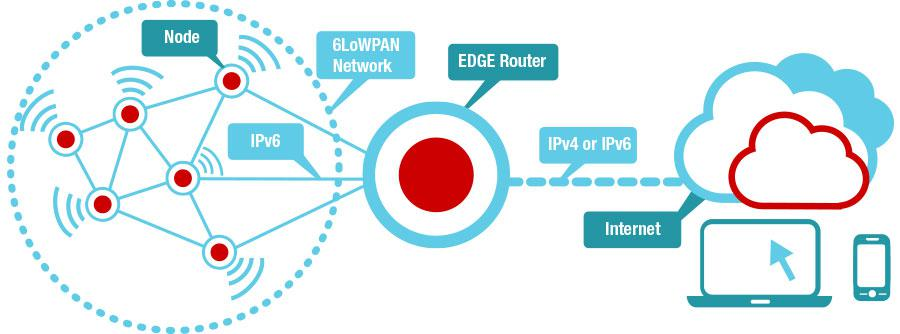
\includegraphics[width=16cm]{images/6lowpan.jpg}
	\caption{Diagramme d'explication de 6LoWPAN.}
	\label{fig:diagramme-6lowpan}
\end{figure}
L'équipe de recherche proposant ce sujet est le groupe 2XS \textbf{eXtra Small eXtra Safe} composée de notamment \textbf{Gilles GRIMAUD} notre encadrant, \textbf{Michael HAUSPIE} son collègue proche de ce sujet et bien sûr le reste de l'équipe.
L'équipe se focalise sur les problématiques de sécurité dans les systèmes embarqués contraints, notamment fournir des solutions logicielles prouvées.

%%% Local Variables: 
%%% mode: latex
%%% TeX-master: "isae-report-template"
%%% End: 

\chapter{Contexte du sujet}
\label{chap:contexte}
%%\begin{itemize}
	%%\item Expliquer le projet
	Notre projet est de produire une sonde qui renifle le trafic réseau dans le contexte de l'Internet des Objets. Cette sonde est un noeud dans ce réseau, et a pour but de transmettre des informations utiles à la sécurisation du réseau, et dans une certaine mesure à l'analyse de ces informations.
%%\end{itemize}

\section{Analyse de l'existant}
	
	\subsection{Internet des objets}
		%%\begin{itemize}
			%%\item Qu'est-ce que c'est ?
		L'Internet des Objets, ou Internet of Things en anglais, correspond à l'extension d'internet aux éléments ou lieux du monde physique, là où l'internet habituel s'arrête au domaine du virtuel.
		Cette technologie est implantée dans notre société avec diverses applications comme la domotique, le médical, la gestion des déchets, mais pas limité à ceux là.
		Notre projet s'inscrit donc dans cet univers puisque les sondes surveillent le trafic de différents éléments d'un sous-réseau d'objets physiques, d'un bâtiment par exemple. \\
		L'Internet des objets regroupe différents modes de communications entre les nœuds d'un réseau tels que le Wi-Fi, le courant porteur ou le bluetooth.%%??definition de 6LowPAN\\
			%%\item Technologies utilisables (bluetooth, wifi, 6lowpan)
			%%Détailler les différentes technologies
		%%\end{itemize}
		
	\subsection{Technologies de communication}
%		\begin{itemize}
%			\item 6lowpan qu'est-ce que c'est ?
%			\begin{itemize}
%				\item définition
		6LoWPAN est une spécification du principe des LoWPAN, c'est à dire un ensemble d'équipements aux ressources limitées, puissance, autonomie entre autres, reliés dans un réseau au débit limité. Typiquement, ces réseaux sont constitués d'un grand nombre d'éléments ou nœuds dans le réseau.
		Basé sur l'IPv6, quelques problèmes se posent avec la spécification standard de celui ci. Ce protocole de communication possède une taille d'entête importante, couplée aux contraintes de tailles de paquets imposées, cela pose des soucis de fragmentation et de réassamblage excessif pour des contrôleurs aux capacités limitées.\\
%				\item exemples (Linky, domotique, industrie)
		La spécification de 6LoWPAN et ses RFC (4919 et 4944) définissent donc des solutions à ces problèmes, et on peut aujourd'hui utiliser plusieurs implémentations de 6LoWPAN, tel que ZigBee. Linky, le nouveau compteur communicant d'ERDF utilise cette technologie. Bien sûr, on peut trouver pléthore de projets et d'objets de domotique se servant de la spécification et de ses implémentations pour communiquer.
		
%			\end{itemize}
%		\end{itemize}
		
	\subsection{Sécurité des communications}
	%		\begin{itemize}
	%			\item Sécurité dans 6lowpan
	%			\begin{itemize}
	%				\item RFC définissent sécurité
		Les différentes RFC définissent un ensemble de consignes sur l'implémentation de la sécurité des réseaux 6LoWPAN notamment sur les différentes couches de la pile protocolaire.
		
		\begin{figure}[htp]
			\centering
			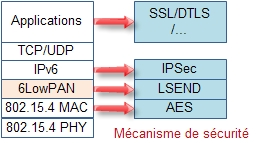
\includegraphics[width=10cm]{images/6lowpan-secu.jpg}
			\caption{Diagramme d'explication de la sécurité des couches de 6LoWPAN.}
			\label{fig:diagramme-6lowpan-secu}
		\end{figure}
		
		\begin{itemize}
			\item Sur la couche MAC : l'algorithme AES doit être utilisé pour sécuriser la couche liaison.
			\item Sur la couche réseau : l'utilisation d'IPsec est possible, mais coûteuse et un échange de clés habituel n'est pas possible. Une extension du protocole SEND -- \emph{\textbf{SE}cure \textbf{N}eighbor \textbf{D}iscovery protocol} -- (RFC 3971) permettant de sécuriser ce mécanisme a été mis en place pour les réseaux 6LoWPAN, appelé LSEND -- \emph{\textbf{L}ightweight \textbf{SE}cure \textbf{N}eighbor \textbf{D}iscovery protocol} --.
			\item Sur la couche application : une solution possible est de mettre en place la sécurisation via SSL.
		\end{itemize}
%				\item Dans les faits, pas vraiment mis en place
		
		Dans les faits, la sécurité étant difficile à mettre en place à cause des contraintes de l'embarqué, elle est parfois insuffisante pour garantir un échange de données sécurisé.
%			\end{itemize}
%		\end{itemize}



\section{Objectif du projet}

	\subsection{Détail du projet}
		%%\begin{itemize}
			%%\item mote qui sniffe, oui mais quoi ?
		Nous avons expliqué l'intitulé du projet mais non pourquoi ces sondes peuvent être utiles. Les sondes sont des noeuds, ou mote dans le jargon de Contiki, qui vont renifler et analyser le trafic circulant, car les informations qu'elles récupèrent permettent la détection d'intrusions. \\
		En effet, le trafic circulant et les paquets sont soumis à des formats spécifiques, contenant des informations qui doivent s'y conformer, ou au contraire faire des écarts vis à vis du format, ce qui constitue une anomalie, et possiblement une attaque.\\
			%%\item système contraint en puissance et en mémoire
		La difficulté de cette analyse réside autant dans les contraintes du matériel, qui est limité en puissance et en mémoire, que dans les solutions mises en places par le réseau pour pallier à ces contraintes, par exemple la compression d'entête.
		%%\end{itemize}
	\subsection{Où s'inscrit le projet ?}
		%%\begin{itemize}
		Comme illustré précédemment, l'Internet des Objets trouve son utilité dans de nombreux domaines. Certains domaines, comme l'industrie ou le médical, font circuler des données sensibles sur le réseau, et des personnes mal intentionnées pourraient causer de graves problèmes sans être détecté si le réseau n'est pas protégé.\\
		Un exemple un peu plus léger est l'histoire du soi-disant hacker qui avait changé le nombre de places des panneaux de parking par des injures. La personne a simplement usurpé l'identité de la machine qui met à jour les places, et a envoyé des paquets falsifiés contenant ces injures.
			%%\item Industrie, hopitaux, mobilier urbain ( pas "simple domotique" )
		%%\end{itemize}

\section{Réponse à un besoin de l'équipe}
	
	\subsection{Focalisation sur la sécurité par 2XS}
%	\begin{itemize}
%		\item Systèmes sûrs
%		\begin{itemize}
%			\item Preuves formelles
		L'équipe de recherche 2XS se focalise sur la création de systèmes sûrs, par le biais de différents mécanismes, dont les preuves formelles de programmes, le développement de librairies, et bien d'autres projets visant à sécuriser les systèmes.\\
		%			\item Différents projets de sécurité
		%		\end{itemize}
		%		\item D'accord, mais quid des communications ?
		
		Mais la problématique de la sécurité ne s'arrête pas à la frontière du système en lui-même, il communique avec d'autres. C'est là que les failles et les fuites d'informations sont les plus nombreuses, même si l'intégrité du système n'est pas en cause.\\
		L'un de leurs projets pour répondre à ce problème est Discus.
%	\end{itemize}
	
	\subsection{Discus}
	Discus est une architecture d'IDS -- Système de détection d'intrusion -- massivement distribuée, qui est configurée grâce à un DSL -- Langage dédié -- Discus-script. Le principe de Discus est d'abstraire la définition des contraintes de sécurité sur un réseau, qu'il soit ethernet, bluetooth ou Wi-Fi.\\
	Notre projet est donc directement en rapport avec celui-ci, fournissant la couche matérielle nécessaire à Discus pour analyser le réseau afin d'y appliquer ces contraintes de sécurité.
%	\begin{itemize}
%		\item IDS -- Système de détection d'intrusion
%	\end{itemize}

\section{Technologies et systèmes utilisés}
	Pour développer notre sonde renifleuse, nous avons utilisé plusieurs outils que nous allons présenter ici :
	
	\subsection{Contiki}
	Contiki est un système d'exploitation léger et flexible avec pour cible les capteurs miniatures en réseau. Ses atouts sont sa flexibilité, sa portabilité, sa faible consommation énergétique, et surtout dans notre cas, son support des protocoles IPv6 et 6LoWPAN. Il répond à une attention importante de la communauté scientifique portée aux réseaux de capteurs sans fil. Il a été créé par une équipe de recherche du centre suédois de recherche scientifique SICS.
	
	\subsection{Outils de simulations}
	Notre sonde a été créée dans un environnement de développement fourni par le site officiel de Contiki, la machine virtuelle InstantContiki3.0, en utilisant principalement pour les tests l'outil de simulation Cooja.\\
	Cooja est un simulateur de matériel pour Contiki permettant de créer virtuellement un réseau de capteurs, de les positionner à notre envie et de charger les différents programmes pour les noeuds (ou motes dans le jargon Contiki) à la volée.
	Nous avons donc passé beaucoup de temps à l'utiliser pour tester notre programme dans des situations réalistes.
	\clearpage
	\begin{figure}[htp]
		\centering
		\includegraphics[width=16cm]{images/cooja}
		\caption{Capture d'écran de Cooja.}
		\label{fig:Cooja}
	\end{figure}

	\subsection{Langage C embarqué et sa chaîne de compilation}
	La création de la sonde s'est fait sur Contiki et le programme a donc dû être adapté aux contraintes du matériel pour lequel il est créé. Pour cela, nous devons rendre le code le plus léger et proche du matériel, et cela passe par l'absence des librairies standard du langage C, par exemple stdlib ou unistd.\\
	La compilation des programmes se fait avec des versions de GCC spécifiques aux architectures matérielles que nous utilisons.
	
	\subsection{Git}
	Git est un gestionnaire de version de projet. Celui-ci permet de synchroniser le travail de notre binôme.\\
	Nous avons choisi d'utiliser la plateforme GitHub pour accueillir notre dépôt Git, afin de faciliter l'accès à notre code.
%%% Local Variables: 
%%% mode: latex
%%% TeX-master: "isae-report-template"
%%% End: 

\chapter{Explications techniques}
\label{sec:technique}

%% CONTIKI =================================================================
\section{Contiki}

	Afin de créer notre sonde, nous avons utilisé Contiki, notamment la Pile réseau IPv6 et les buffers cycliques.
	
	\subsection{Pile réseau de Contiki}
	
		Contiki possède trois piles réseau :
		\begin{itemize}
			\item Rime
			\item IPv4
			\item IPv6
		\end{itemize}
		Bien évidemment, celle qui nous intéresse ici est la pile IPv6. 
		
		\subsubsection{Organisation de la pile IPv6}
			
			L'implémentation de la pile réseau nous permet d'utiliser les communications avec aisance. C'est grâce à elle que nous pouvons envoyer et recevoir des messages.
			
			La pile réseau se découpe en quatre couches :
			\begin{itemize}
				\item Couche réseau
				\item Couche MAC -- Medium Access Control
				\item Couche RDC -- Radio Duty Cycling
				\item Couche radio
			\end{itemize}
			
			\clearpage
			
			\begin{figure}[htp]
				\centering
				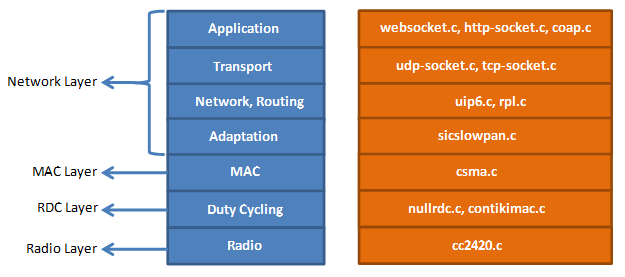
\includegraphics[width=16cm]{images/Contikinetstack}
				\caption{Organisation de la pile réseau de Contiki.}
				\label{fig:contikinetstack}
			\end{figure}
			
		\subsubsection{Packetbuf}
		
			Pour envoyer et recevoir des paquets, Contiki se base sur un buffer unique de paquets -- paquetbuf, qu'ils soient entrants ou sortants.
			Le buffer est découpé en deux parties, la première pour l'en-tête, et la deuxième pour les données.
			
			\begin{figure}[htp]
				\centering
				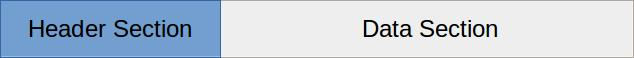
\includegraphics[width=12cm]{images/Buf.jpg}
				\caption{Découpage du buffer de paquets de Contiki.}
				\label{fig:buf}
			\end{figure}
			
			Une différence est faite entre les paquets sortants et les paquets entrants.
			
			\clearpage
			\begin{figure}[htp]
				\centering
				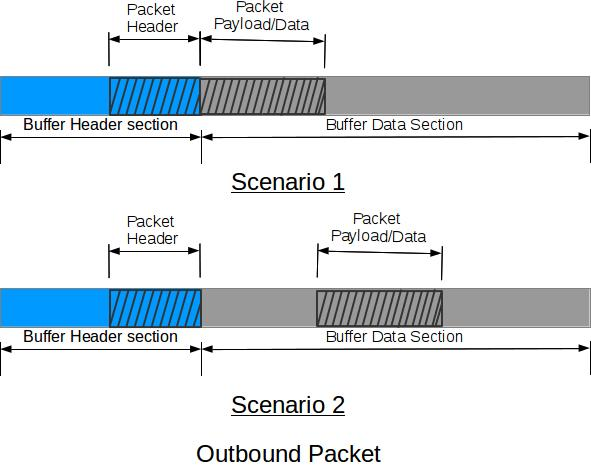
\includegraphics[width=13cm]{images/Out.jpg}
				\caption{Répartition des données pour un paquet sortant.}
				\label{fig:outbuf}
			\end{figure}
			
			
			Le buffer pour les paquets sortants permet de construire ce qu'on veut envoyer de façon structurée, avec une séparation de l'en-tête et des données qui permet de modifier l'un sans influer sur l'autre. \\
			Ce découpage donne accès aux attributs des paquets, ce qui comprend 4 niveaux d'utilisations :
			\begin{itemize}
				\item Local
				\item Entre deux voisins
				\item Entre les noeuds en bout de la communication
				\item L'expéditeur et le receveur locaux, et l'expéditeur et le receveur finaux
			\end{itemize}
			Ces attributs sont toutes les informations utiles à la diffusion et au routage du paquet, par exemple le canal, le numéro de séquence, le nombre de sauts, et bien d'autres, 26 au total.
			
			\clearpage
			
			\begin{figure}[htp]
				\centering
				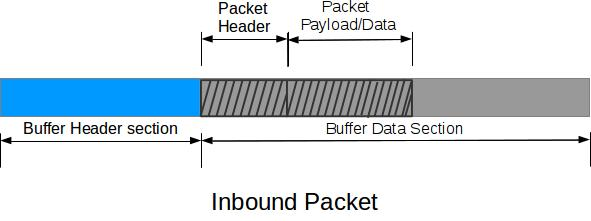
\includegraphics[width=13cm]{images/In.jpg}
				\caption{Répartition des données pour un paquet entrant.}
				\label{fig:inbuf}
			\end{figure}
			
			Le buffer pour les paquets entrant ne fait pas la différence entre en-tête et données, et met tout dans la partie données. Cela permet d'économiser de la puissance de calcul en évitant d'interpréter l'en-tête.\\
			Les fonctions à disposition permettent uniquement de récupérer le paquet brut. Pour effectuer nos vérifications, ils nous faut donc étudier la construction des paquets.
	
	\subsection{Systèmes de stockage Contiki}
		
		Pour nos vérifications superficielles, il nous a été demandé de stocker temporairement quelques informations à propos des paquets du trafic. Nous avons considéré plusieurs options pour stocker ces informations.

		\subsubsection{Contiki Coffee file system}
%			\begin{itemize}
%				\item Expliquer comment écrire dedans
			Contiki possède plusieurs systèmes de fichiers qui implémentent l'interface de Contiki File System, dont Coffee. Coffee est utilisé sur les appareils équipés avec de la mémoire flash ou de l'EEPROM. Contiki s'occupe de l'implémentation matérielle, et Coffee fournit une API qui est similaire aux opérations sur les fichiers du langage C standard.\\
			
%				\item Expliquer pourquoi on ne l'a pas utilisé
			L'intérêt d'un système de fichier est d'envoyer d'un seul coup plusieurs données, afin de limiter le nombre de transmissions, et donc de consommer moins d'énergie. Aussi, garder les données en mémoire de façon locale permet, en cas de transmission échouée, de ne pas les perdre définitivement.
			
			Nous avons préféré nous tourner vers la mémoire volatile pour enregistrer les informations, pour avoir une solution moins lourde.
%			\end{itemize}
		\subsubsection{Volatile}
			
			La mémoire volatile de Contiki peut s'utiliser de plusieurs façons :\\ \\
			\textbf{Listes}\\
%			\begin{itemize}
%				\item Expliquer comment écrire dedans
				La librairie de Contiki pour les listes procure une liste chaînée dans laquelle les informations souhaitées sont stockées puis récupérées par la suite. La librairie est utilisée partout dans Contiki pour stocker les listes des processus, les files de paquets, les listes des voisins, et d'autres tables.\\
				\begin{figure}[htp]
					\centering
					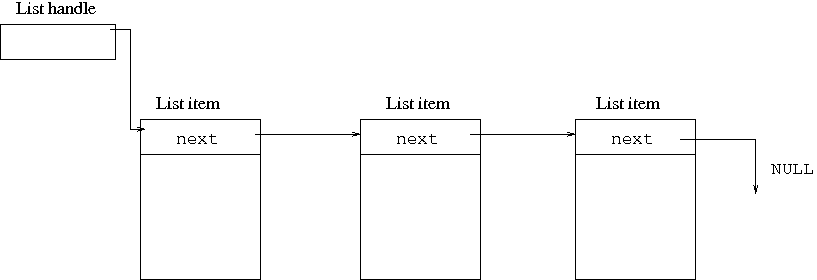
\includegraphics[width=16cm]{images/linked-list}
					\caption{Architecture d'une liste chaînée sur Contiki.}
					\label{fig:list}
				\end{figure}
				Les objets de la liste sont des structures qui sont définies par le modules qui utilise la liste. La seule condition est que le premier objet de la liste doit être un pointeur, qui est utilisé par la librairie pour lier les objets ensemble dans la liste.\\
				Une liste de Contiki consiste d'un pointeur et de zéro ou plus objets dans la liste, comme montré dans l'illustration ci-dessus. Le pointeur pointe vers le premier objet de la liste.\\
				
				La liste était l'une des solutions potentielles à notre besoin de stockage, mais il a été décidé de faire appel à un moyen encore plus léger : le buffer cyclique.
%				\item Expliquer pourquoi on ne l'a pas utilisé
%			\end{itemize}
			\clearpage
			\textbf{Buffers cycliques}\\
%			\begin{itemize}
%				\item Expliquer comment écrire dedans
				Il y a plusieurs endroits dans Contiki où un gestionnaire d'interruption doit garder des données qui peuvent être indépendamment être lues par d'autres parties de Contiki. Le gestionnaire et les fonctions de lectures doivent être synchronisées pour éviter les problèmes de concurrence, parce le gestionnaire peut préempter les parties qui lisent les données à n'importe quel moment. Les mécanismes de lecture et d'écriture sont donc pensées pour être indépendantes de chacune.\\
				\begin{figure}[htp]
					\centering
					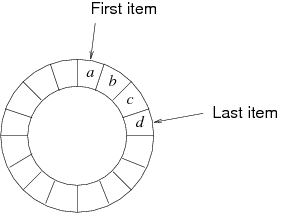
\includegraphics[width=10cm]{images/ringbuf}
					\caption{Architecture d'un buffer cyclique sur Contiki.}
					\label{fig:ringbuf}
				\end{figure}\\
%				\item Expliquer pourquoi on l'a utilisé
%			\end{itemize}
				Ci-dessus : Un buffer cyclique avec quatre objets, a, b, c et d. L'objet a est le prochain a sortir du buffer. Le d est l'objet le plus récemment inséré. Le premier et dernier pointeur permettent d'y accéder respectivement.\\\\
				Un buffer cyclique ( parfois appelé buffer en anneau ) est une structure de données qui garde les données en mémoire sous la forme d'un anneau comme montré ce-dessus. Les données sont stockées dans le buffer, et sont lues dans le même ordre que celui dans lequel elles ont été insérées. La structure est donc proche d'une FIFO ( First In First Out ) ou file en français, mais avec la particularité d'être cyclique.\\
				%The Contiki ring buffer library implements a ring buffer handling mechanism that stores bytes in an array that must have a size that is a powers of two, and 256 bytes or less. The reason for requiring that the size is a power of two is that wrapping of the first and last pointer in the ring structure can be implemented using bit-wise Boolean operators.
				Contiki propose une librairie qui implémente les buffers cycliques, qui garde en mémoire des octets dans un tableau dont la taille doit être une puissance de deux, inférieure ou égale à 256. La raison pour la contrainte sur les puissances de deux est que la structure implémente les fonctions sur les pointeurs de début et de fin avec des opérateurs booléens.\\
				Aussi, la taille maximale de 256 octets est là pour permettre à ces pointeurs de début et de fin de tenir dans une structure de 8 bits. L'octet habituel est la seule structure de donnée qui peut être mise à jour de façon atomique, ce qui est important pour assurer la synchronisation entre les lectures et écritures sur le buffer cyclique, même si l'un préempte l'autre.\\
				
				Malgré les contraintes imposées par cette structure, sa légèreté et ses propriétés de synchronisation sont des gros avantages sur les autres structures : Les paquets n'attendent pas que Contiki ait fini d'écrire dans sa mémoire.
	
%% 6LoWPAN =================================================================
\section{6LoWPAN}
	\subsection{Compression des headers}
%		\begin{itemize}
%			\item Pourquoi compresser ?
		Comme évoqué dans l'analyse de l'existant, les communications via IPv6 se révèlent peu pratiques pour des systèmes contraints, surtout à cause des headers ( ou entêtes ) trop volumineux qui réduisent la charge utile de données contenues par un paquet, multipliant le nombre de paquets. \\
		La RFC 4944 définit LOWPAN\_HC1, le mécanisme de compression des en-têtes IPv6 pour les LowPAN. Elle intègre aussi la compression de l'en-tête UDP sur 4 octets, mais n'autorise pas la compression du Checksum. De plus, elle restreint la plage des ports UDP de 61616 à 61631 afin de compresser à 4 bits cette valeur.
		
		\begin{figure}[htp]
			\centering
			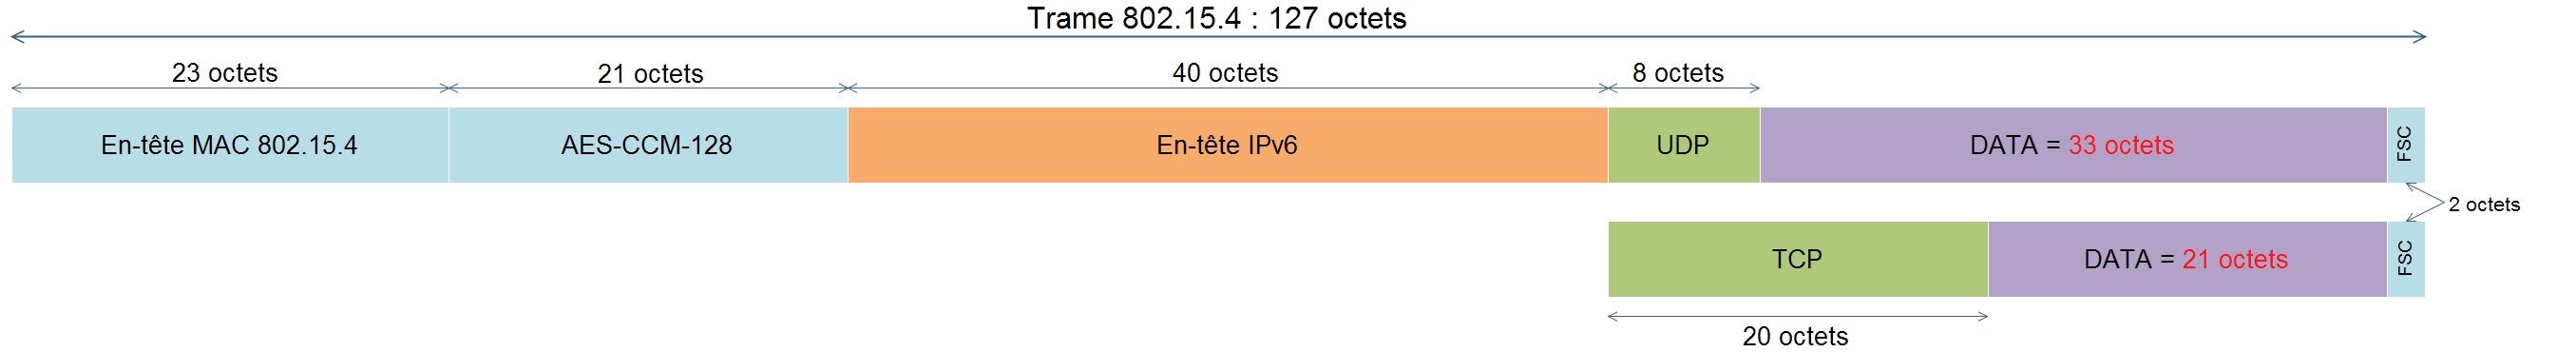
\includegraphics[width=16cm]{images/TramePasComp.jpg}
			\caption{Trame IPv6 non compressée.}
			\label{fig:tramepascomp}
		\end{figure}
		
		\begin{figure}[htp]
			\centering
			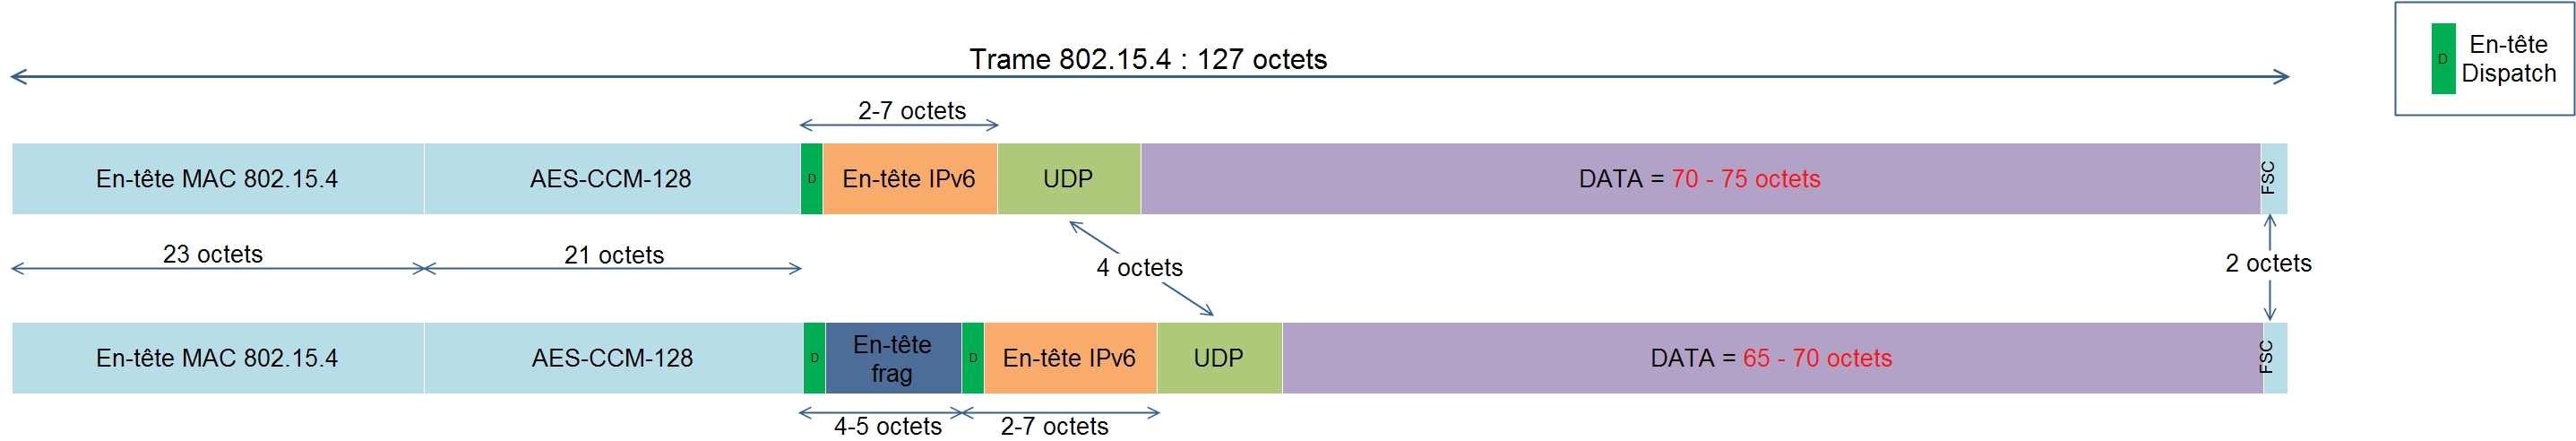
\includegraphics[width=17cm]{images/TrameComp.jpg}
			\caption{Trame IPv6 compressée.}
			\label{fig:tramecomp}
		\end{figure}
		On remarque que la charge utile est doublée grâce à la compression d'en-tête.
%			\item Comment ça marche ( avec images )
%		\end{itemize}
%	
	\subsection{Attaques possibles}
		Notre but étant de travailler vers la sécurisation d'un réseau 6LoWPAN, nous avons étudié différentes attaques possibles sur ce type de réseau. Elles se classent en deux catégories : Celles qui sont pertinentes pour notre sujet, et celles qui ne le sont pas.\\
		
		\subsubsection{Non-pertinentes}
%	\begin{itemize}
%		\item Qui nous intéressent pas directement
%		\begin{itemize}
%			\item Attaques passives ( écoute )
%			\item Brouillage des ondes
%			\item Inondation de paquets
%		\end{itemize}
			Les attaques passives telles que les écoutes, les attaques de brouillage des ondes, ou d'inondation de paquets sont difficilement repérables par un noeud du réseau. Ces attaques ne sont donc pas pertinentes dans le cadre de notre sujet, car il faudrait fait usage de matériel différent de nos capteurs.
		\subsubsection{Pertinentes}
%		\item Qui nous intéressent
%		\begin{itemize}
%			\item Spoofing
%			\item Paquets dupliqués
%			\item Paquets fabriqués
%			\item Sybil attack
%		\end{itemize}
			D'autres attaques, comme la duplication ou falsification de paquets, le spoofing et l'attaque Sybil sont des exemples que nous avons étudié pour préparer des vérifications sur notre capteur.\\
			
			La \textbf{falsification} de paquets peut entrainer une nombre de situations d'attaque, tout en étant difficile à détecter. Un paquet peut être falsifié sur plusieurs champs ou un seul, pour avoir différents effets.\\
			Le \textbf{spoofing} est la situation où un attaquant envoie un paquet en falsifiant l'adresse source pour se faire passer pour quelqu'un d'autre, généralement une adresse de confiance.\\
			La \textbf{duplication} de paquets est une autre manière de mener une attaque contre un réseau, par exemple, en renvoyant un message d'authentification antérieur.\\
			L'\textbf{attaque Sybil} est particulière, il s'agit d'un seul acteur possédant plusieurs identités, par exemple un seul noeud qui envoie des messages avec deux ou plus adresses sources qui n'étaient pas utilisées auparavant. C'est ce qui la différencie d'un simple spoof.
%	\end{itemize}
%	Nos possibles solutions du coup


%%% Local Variables: 
%%% mode: latex
%%% TeX-master: "isae-report-template"
%%% End: 

\chapter{Déroulement du projet}
\label{sec:deroulement}

\section{Prise en main du sujet et des technologies}
	Après ces explications techniques, il est temps d'expliquer comment le projet s'est déroulé pour nous. Au début, il nous a fallu prendre en main les différents outils pour travailler.
	
	\subsection{Contiki}
	Comme nous avons déjà vu, Contiki est un système d'exploitation qui vise les systèmes embarqués. Notre expérience avec l'embarqué était limitée bien que non-nulle, aussi la prise en main s'est faite assez rapidement, même si difficilement.\\
	Certains concepts, comme les proto-threads utilisés par Contiki, sont assez proches d'autres concepts présents dans les systèmes d'exploitation habituels, néanmoins la découverte des fonctionnalités de Contiki a pris du temps car il est complet et offre les principales caractéristiques et fonctionnalités d'un système habituel.\\
	Ceci est l'une des raisons, avec celles déjà évoquées pour IPv6 et 6LoWPAN, du choix de Contiki plutôt que FreeRTOS ou TinyOS, qui peuvent avoir plusieurs de ces caractéristiques, mais Contiki les assemble toutes.
%		\begin{itemize}
%			\item Embarqué
%			\item simulations avec Cooja
%			\item Pourquoi Contiki et pas un autre ?
%		\end{itemize}

	\subsection{Chaîne de compilation et pilotes}
	Les découvertes ici ont été plutôt rapides puisque la machine virtuelle InstantContiki3.0 contient la chaîne de compilation nécessaire à la compilation des projets sur les différentes architectures supportées par Contiki. L'installation à la main de la chaîne de compilation est bien documentée sur les différents tutoriels concernant Contiki présents sur Internet.\\
	Les pilotes des différents contrôleurs radios sont par contre difficiles à prendre en main, aussi avons nous choisi de nous concentrer sur les contrôleurs cc2420 de Texas Instrument car déjà présent dans d'autres projets que nous avons passés en revue.
%		\begin{itemize}
%			\item GCC
%			\item architectures différentes
%			\item contrôleurs radio différents
%		\end{itemize}

\section{Programme développé}
	\subsection{Fonctionnement du projet}
	\subsection{État du projet}

\section{Retours d'expérience} % DONE ?
    Pendant ce projet, nous avons pu apprendre beaucoup de choses, développer nos compétences et de produire un programme, dont qui peut bénéficier d'évolutions sur le court et long terme.
    
	\subsection{Évolutions à court terme} % DONE
	A court terme, il est évidemment possible d'ajouter d'autres détections d'attaques en fonction des besoins, mais ce qui est le plus utile à l'équipe de recherche est d'intégrer notre sonde dans Discus, leur système de détection d'intrusion.
	La sonde peut fournir les informations dont Discus a besoin pour faire respecter les contraintes énoncée dans le script adéquat. 
	Les vérifications d'attaques sont donc effectée par le système qui reçoit les informations, et non par les sondes directement, ce qui allège la charge de travail sur les capteurs aux capacités restreintes. Aussi, les nouvelles vérifications d'intrusion pourront s'écrire et se faire sans reprogrammer les sondes.
	\subsection{Évolutions à long terme} % DONE
	Sur un plus long terme, il a été pensé d'éventuellement faire communiquer les sondes entre elles afin de créer une grille de capteurs.
	Cela permettrait, grâce aux différents RSSI pour un seul paquet captés par les sondes, de localiser les différents acteurs du réseau, et donc de localiser l'attaquant lors d'une anomalie.
	\subsection{Challenges} % DONE
	    Ce projet a été très intéressant et instructif, mais nous avons dû faire face à plusieurs difficultés et challenges lors de son déroulement. Bien que ces contraintes aient pu parfois nous ralentir, elles furent instructives à plusieurs niveaux.\\
	    Tout d'abord, le sujet du projet se concentre sur des domaines et technologies dont nous n'étions pas très familiers. Le monde de l'informatique embarquée est fait de contraintes auxquelles il faut s'adapter pour être productif, les retours beaucoup moins verbeux lors d'erreurs, les limites de mémoire, de puissance, et parfois l'absence de librairies pour rendre le code assez léger pour la plateforme sont quelques exemples de difficultés lorsqu'on découvre l'embarqué. S'y adapter n'est pas un obstacle en soi, mais il faut bien se préparer et ne pas avoir peur de prendre son temps pour cela.\\
	    Les découvertes étaient nettement plus nombreuses dans les technologies employées, notamment au niveau des systèmes d'exploitation embarqués, comme Contiki, et leurs technologies de communication. Nous avons lu beaucoup de spécifications, de RFC et de documentation, et en rétrospective, nous aurions eu plus de facilité à établir un plan d'approche, organiser nos découvertes pour éviter la confusion. Par exemple, prendre du temps pour bien se renseigner sur Contiki, puis lorsque l'outil est maîtrisé, se renseigner sur 6LoWPAN, et ainsi de suite.\\
	    Malgré nos recherches en profondeur, nous sommes parfois tombés sur des incohérences dans la documentation, ou des explications pas assez claires, notamment sur le buffer de paquets qui traite différemment les paquets réseau selon qu'ils soient entrants ou sortants. Pour pallier à ce souci, nous avons recherché plus d'informations sur des sites et des encyclopédies en ligne (wikis) universitaires qui se sont penchés sur Contiki et ont écrit de bons tutoriels.\\
	    Parfois, certains exemples de code présents dans Contiki ne sont pas assez commentés, ce qui peut être problématique pour apprendre comment certains programmes sont faits. C'est pourquoi il ne faut pas hésiter à rechercher sur des forums des discussions traitant de ces sujets et à contacter certains interlocuteurs pour demander de l'aide.

%%% Local Variables: 
%%% mode: latex
%%% TeX-master: "isae-report-template"
%%% End: 

\chapter*{Conclusion et perspectives}
\addcontentsline{toc}{chapter}{Conclusion}
\markboth{Conclusion}{Conclusion}
\label{sec:conclusion}

    %Conclusion et ouverture
	%\item Résumer le sujet, sa problématique et notre morceau de solution
    Notre sujet de projet était de contribuer à un système de détection d'intrusion pour l'Internet des Objets.
    La principale difficulté de ce sujet était les nombreuses attaques possibles sur le réseau, notamment le détournement de routage pour l'écoute, le vol d'identité et la falsification de paquets. En partant de cette problématique, nous avons produit une sonde, un noeud sur le réseau qui écoute le trafic radio, afin de construire par dessus plusieurs couches de détections.\\
	%\item Ce qu'on a apporté
    De ce fait, nous procurons à l'équipe de recherche les prémisses d'un outil de base pour développer la sécurité réseau dans l'IDS de l'équipe -- Discus, en rajoutant la plateforme radio aux autres déjà existantes.\\

	%\item Ce que ça nous a apporté
	En travaillant sur ce projet, nous avons pu découvrir des technologies que nous n'avons pas l'habitude de voir lors de nos cours. Cela nous a permis d'élargir nos horizons vis à vis des domaines de l'informatique, de tester de nouveaux paradigmes.\\
	%\item Comment ce qu'on a appris va nous servir plus tard
	Nous avons pu nous améliorer sur notre travail en autonomie, nous entraîner à la recherche d'information, de documentation. Cet entraînement est aussi un regard vers ce qu'est le monde de la recherche, qui a permis de le découvrir ou le redécouvrir.
	
	% TODO

%%% Local Variables: 
%%% mode: latex
%%% TeX-master: "isae-report-template"
%%% End: 



\clearpage

\end{document}